\documentclass[12pt, titlepage]{article}

\usepackage[sumlimits,nointlimits,namelimits]{amsmath}
\usepackage{amsfonts}
\usepackage{amssymb}
\usepackage{mathtools}
\usepackage[shortlabels]{enumitem}
\usepackage{graphicx}

\usepackage[utf8]{inputenc}
\usepackage[T1]{fontenc}
\usepackage{lmodern}
\usepackage[margin=1in]{geometry}
\usepackage{fancyhdr}
\usepackage[dvipsnames]{xcolor}
\usepackage{tikz}

\setlist[itemize]{topsep=0pt}
\setlist[enumerate]{topsep=0pt, label=(\alph*)}

\setlength\parindent{0pt}
\setlength\parskip{6pt}

\renewcommand{\headrulewidth}{0pt}
\fancyhead[L]{\bf CS 452/652}
\fancyhead[C]{\bf Kernel Assignment 3}
\fancyhead[R]{\bf Heun \& Yao}

\usepackage{hyperref}

\hypersetup{
    pdftitle={Kernel Assignment 3}
    colorlinks=false,
    pdfborder={0 0 1.5},
    linkbordercolor=red,
    urlbordercolor={0 1 1}
}

\begin{document}
    \begin{titlepage}
        \begin{center}
            \vspace*{5em}
            \textbf{\LARGE Kernel Assignment 3}
            \vspace*{3em}

            \begin{tabular}{c@{\hskip 8em}c}
                \textbf{\large Niclas Heun} & \textbf{\large Trevor J. Yao} \\
                {\small nheun@uwaterloo.ca} & {\small t27yao@uwaterloo.ca} \\
                {\footnotesize 21111245} & {\footnotesize 20830290} \\
            \end{tabular}

            \vfill

            Professor Ken Salem \\
            CS 452/652: Real-Time Programming (Fall 2023) \\
            University of Waterloo \\
            19 October 2023

            \vspace*{5em}

        \end{center}
    \end{titlepage}


    \pagestyle{fancy}

    \tableofcontents
    \pagebreak

    \section{Overview}
    \label{sec:overview}

    This assignment begins the implementation of the Train Control Kernel in order to enable a task-based parallelism model for task management. The end goal is to enable more complex train-control, which would not be possible with a single sequential thread of execution, as used in A0.

    For this assignment, there is no interactive interface. The Kernel starts up and executes the user-level entrypoint function \verb`void user_main(void)`. The User level programs required for each assignment are found in \verb`user/includes/kX.h`, where \verb`X` is the assignment number, and the entrypoint executes the specified user programs.

    \subsection{Submission SHAs}

    The repository for the kernel is \href{https://git.uwaterloo.ca/t27yao/cs452-kernel}{ist-git@git.uwaterloo.ca:t27yao/cs452-kernel.git}. The submission SHAs for their respective assignments are listed below:
    \begin{itemize}
        \item A1: 6a8841836fc9ce629b573e94b37c901b4d71f2ee;
        \item A2: f284ab2f8195101c9d9bdd1c908a8abfd07324c3;
        \item A3: $\langle$hash$\rangle$.
    \end{itemize}

    \section{Execution}

    Build the program from the root directory by running one of \verb`make` or \verb`make all`. The specific user-level programs for each assignment can be built by specifying the target \verb`make kX`, where \verb`X` is the assignment number. It may be necessary to set the \verb`XDIR` variable to point to the directory containing the cross-compiler. For example, in the \verb`linux.student.cs` environment, \verb`XDIR` should be \verb`/u/cs452/public/xdev` (i.e. the parent of the \verb`bin` directory). Therefore, the program can be compiled in the \verb`linux.student.cs` environment by changing directory to the program root and executing:
    \begin{verbatim}
make XDIR=/u/cs452/public/xdev
    \end{verbatim}

    \subsection{K2 Test Programs}
    The RPS Game and Performance measurements programs required for K2 are built using the targets \verb`k2` and \verb`k2-timings` (i.e. the default \verb`k2` target will build the RPS Game).

    \section{Kernel Structure}

    The program files are structured into three parts -- Kernel, User Libraries, and User. These parts each have their own directories, \verb`kernel/`, \verb`./` (i.e. the repository root), and \verb`user/` respectively. In each of these directories, the header and implementation files are split into the directories \verb`includes` and \verb`src` respectively.

    \subsection{Generic Kernel Loop}
    \label{sec:main}

    The kernel is designed as a generic loop, rather than as an event handler. As part of the initialisation, the kernel performs a number of tasks:
    \begin{enumerate}[(1)]
        \item Initialise singleton data structures for task/stack allocation, scheduling, interrupt handling, and timing;
        \item Initialise the initial kernel state for context switching;
        \item Install the address of the exception vector into the \verb`VBAR_EL1` system register;
        \item Initialise the UARTs;
        \item Allocate and initialise the nameserver;
        \item Allocate and initialise the first user task (with default entrypoint \verb`user_main`).
        \item Allocate and initialise the idle task.
    \end{enumerate}

    Then, on each iteration of its main loop, the kernel does the following:
    \begin{enumerate}[(1)]
        \item Remove the next task from the queue as given by the scheduling algorithm (Section \ref{sec:scheduling});
        \item Context switch (Section \ref{sec:context-switch}) into the selected task;
        \item On execution and handling by the hardware of the \verb`svc N` instruction or interrupt, context switch back to the kernel, returning the handler.
        \item Based on the handler, handle the system call (Section \ref{sec:sys-calls}) or interrupt (Section \ref{sec:interrupt}) as described in the interface.
    \end{enumerate}

    The kernel loop ends when all created user tasks (including the initial task) has exited, and restarts the machine.

    \subsection{Critical System Parameters and Limitations}
    \label{sec:limits}
    The stack size is limited to \verb`0x80000` bytes, or 512 KiB per task. The maximum number of simultaneous running tasks is 1024. These numbers were chosen because they provide a modest stack size while allowing the possibility of a large number of simultaneously running smaller tasks, and both being powers of 2 ($2^{19}$ and $2^{10}$ respectively) to allow for faster calculations. In total, this gives the program 500 MiB to work with in total task stack size, which, taking into account that we have approximately 1 Gb of program memory to work with, and leaving room for the bootloader and the program load address of \verb`0x80000`, gives more than enough room.

    The TIDs are limited by the address space of \verb`uint16_t`, i.e.\ 65,535 TIDs. This is far more than the total number of tasks, while being reasonably space efficient. The TIDs are reassigned, and the algorithm for this is discussed in Section \ref{sec:tids}. The larger address space for TIDs compared to the number of simultaneous active tasks is to prevent more expensive reassignment searches from occurring frequently.

    The nameserver names are limited in length to 256, since without heap allocation dynamic arrays are not really possible, nor necessary. It is incredibly unlikely that names will be longer than 256 characters, and if so, the user programmer should seriously reconsider a better naming scheme. The maximum number of names the nameserver can hold is also 256, since it is reasoned that most tasks do not need to be known, and thus being able to hold a quarter of tasks in the nameserver is more than enough.

    \subsection{Algorithms}

    \subsubsection{Context Switching}
    \label{sec:context-switch}

    Context switching is implemented in \verb`kernel/src/context-switch-asm.S` as an assembly routine linked as a C routine. On boot, the kernel starts first and creates an entrypoint user-level task, and context switches it via the following routine:
    \begin{verbatim}
void context_switch_out(task_t *curr_user_task, kernel_state *kernel_task);
    \end{verbatim}
    This assembler routine pushes the addresses of the task descriptors onto the stack (important for context switching back into the kernel). It then uses \verb`x0` to point to the beginning of the \verb`kernel_task`, and directly stores registers \verb`x1` to \verb`x30` into the state using offsets of \verb`x0`. It then lastly takes \verb`x0` which was stored onto the stack and saves it into the state. Next, the routine has to load the saved registers of the user task. It does so again by using \verb`x0` and \verb`x1` as scratch registers, loading the address of \verb`curr_user_task` into \verb`x0` from the stack. First, it directly loads registers \verb`x2` to \verb`x30` using offsets of \verb`x0`. It then loads the \verb`pc` into \verb`ELR_EL1`, \verb`sp` into \verb`SP_EL0`, and the saved \verb`pstate` into \verb`SPSR_EL1`, taking care to only load 32 bits. After this, it then loads registers \verb`x1` and \verb`x0`, in that order, since we used them as scratch registers.

    Context switching in is much the same but in inverse, but makes use of the fact that after the \verb`svc` instruction is executed, we are on the kernel stack, and thus is able to re-save the user task and restore the kernel task. However, before storing the user task, we need to push any registers we need as scratch (i.e. \verb`x0`) onto the stack before doing anything else, and rewrite it to the task descriptor at the end.

    \subsubsection{Stack Allocation}

    User level stacks are allocated in memory following the kernel stack, with the previously discussed constraints in Section \ref{sec:limits}. Stack allocation is managed by the singleton \verb`stack_alloc` structure defined in \verb`kernel/include/stack-alloc.h`. They are allocated in linear fashion after the kernel stack, but not zeroed out to increase performance of task creation, since there was a significant lag when clearing a stack size of 512 KiB. Freed task stacks are reclaimed linearly to reduce fragmentation. It was considered to use slab allocation to better reduce fragmentation, but the overhead for managing this does not seem worth it at this time. If we see fragmentation later on when working with more tasks, this change will be made.

    \subsubsection{Task Allocation}
    \label{sec:task-alloc}

    The task allocation mechanism employs a sophisticated slab allocation strategy to optimise memory usage and mitigate memory fragmentation.
    Initially, the memory is segmented into 128 slabs, each containing 8 tasks.
    Whenever the free list is exhausted, a new slab is initialised, with its 8 tasks added to the free list and the slab marked as active.
    To track the usage, a counter is associated with each slab to monitor its active status and the number of used tasks;
    additionally, every task contains a variable to indicate the slab it belongs to.

    When a task is added back to the freelist, it is not just added to the front of the free list.
    Instead, the free list is structured by slab-id, ensuring the utilisation of lower slabs first.
    When all tasks from a specific slab are added back to the free list, and consequently, the task usage counter for that slab resets to zero, all tasks from that slab are extracted from the free list and the slab is deallocated.
    If again additional memory is required, the lowest unused slab is (re)activated and its tasks are (re)integrated into the free list.
    This procedure ensures minimal fragmentation and optimal utilisation of available memory.
    This is also less expensive to do than other algorithms, such as precisely tracking allocations in a separate structure.

    \subsubsection{Task IDs}
    \label{sec:tids}

    The task ID (TID) allocation is inspired by the algorithm UNIX uses for allocating process IDs. TIDs are allocated sequentially to tasks until they reach the maximum TID value (65,535), in which allocation returns to 300 and increases again. This is used because it is less likely that long running tasks were allocated with higher TIDs, and can obviously be adjusted in the future as we see fit to increase performance.

    On each choice of TID, the kernel checks that the TID is not in use, and if so tries the next one. This is obviously worst-case expensive, but as mentioned previously, the large TID space in comparison to the number of tasks makes the search unlikely to be long. The slight increase in cost per task allocation is marginal, and if it works for UNIX, it works for us.

    User tasks are allocated beginning with TID 50, since we know there will be longer running server tasks that are started by the kernel.

    The Task ID algorithm is implemented in the static \verb`task_queue_get_tid` method located in \verb`kernel/src/task-queue.c`.

    \subsubsection{Scheduling}
    \label{sec:scheduling}

    The scheduling follows a straightforward round-robin approach, housed within the task queue.
    Starting with the highest priority queue, it cycles through the queue to return the first task in a \verb`STATE_READY` condition.
    Tasks not in ready state are skipped and maintain their position within the queue.
    Should the queue be empty or only comprise of non-ready tasks, the scheduler advances to the next lower priority queue in search of ready tasks.
    New tasks are always added to the end of their respective priority queue.

    Long running server tasks which are started in the kernel initialisation have their own highest priority, in order to enable timely service to user tasks. These tasks are excluded when checking for active user tasks, and are user tasks with special treatment. 
    
    If any of these server tasks require notifier task(s), they also can be run at a higher priority (under the server tasks), which are also excluded when checking for active user tasks. Finally, the idle task (Section \ref{sec:idle-task}) runs at the lowest priority without any other tasks, and is also ignored to allow for smooth exit. In essence, any server/kernel tasks are always ignored.

    \subsubsection{System Calls}
    \label{sec:sys-calls}

    The individual System Calls implemented for this assignment (\verb`Create`, \verb`Exit`, etc) are implemented in \verb`includes/task.h`. These methods are simply a wrapper on the \verb`syscall` procedure implemented in \verb`includes/syscall.h`. This method takes advantage of the compiler moving call arguments into registers \verb`x0` to \verb`x7`, and simply calls \verb`svc #0`, with the syscall number being stored as the first argument, and then returns (when the kernel eventually switches us back as the active task).

    These arguments are preserved during the context switch, and saved in the task descriptor for processing. During this, the kernel executes code based on the syscall number in \verb`x0`, and returns the result (if any) in \verb`x0`, following aarch64 convention. This means that when the application is switched back, and returns to the location of the \verb`svc` instruction, it will return the value in \verb`x0`.

    \subsubsection{Message Passing}
    \label{sec:msg-passing}

    Message passing is implemented as part of three methods: \verb`Send`, \verb`Receive`, and \verb`Reply`. These are defined in the header \verb`include/msg.h`, and are implemented as system calls (Section \ref{sec:sys-calls}. All together, these form the message passing algorithm, which allows user tasks to communicate between each other. For our discussion we will denote $T_s$ and $T_r$ be the sending and receiving task respectively. For the sending and receiving sections, we will discuss the algorithm in two cases, depending on which task executes first.

    First, suppose $T_s$ executes first. When $T_s$ executes \verb`Send`, it blocks until after $T_r$ has called \verb`Reply`, which is accomplished by the kernel moving $T_s$'s ready state from \verb`READY` to \verb`SEND_WAIT`. It then attaches $T_s$ to the back of $T_r$'s waiting queue, which is implemented as an intrusive linked list, and is separate from the task scheduler (i.e. tasks stay on the scheduler queue even if they are in a task's waiting queue). Note that the kernel can easily determine that $T_s$ was called first by checking the ready state of $T_r$ (i.e. in this case, $T_r$ will be \verb`READY`, rather than \verb`RCV_WAIT`). Next, when $T_r$ calls \verb`Receive`, the kernel knows $T_s$ went first since its waiting queue is not-empty, and pops $T_s$ of the waiting queue. It then moves $T_s$ to state \verb`RPLY_WAIT`, and copies the necessary bytes (i.e. the minimum) between the given buffers, and returns the necessary information as in any system call. Note that since $T_r$ needs to handle the receive, the kernel does not block it.

    Secondly, we will consider the case for when $T_r$ executes first, which the kernel can recognise if there are no waiting senders. In this case $T_r$ is blocked by the kernel moving it to the \verb`RCV_WAIT` state. Then, when $T_s$ sends, the kernel blocks it and transitions it to state \verb`RPLY_WAIT`, and moves the data as before. However, in this case, the kernel has to unblock $T_r$ (i.e. ready state to \verb`READY`) before returning the necessary parameters as previous. As mentioned previously, the kernel is able to check that $T_r$ executed first by verifying that $T_r$ is in \verb`RCV_WAIT` state.

    In either case, $T_r$ processes the sent message, and needs to \verb`Reply` to $T_s$. The kernel handles this by copying the appropriate number of bytes, and unblocks $T_s$ by returning it to the \verb`READY` state.
    
    \subsubsection{Interrupts}
    \label{sec:interrupt}
    Interrupts are set-up and handled (i.e. acknowledgement, etc) as documented in the ARM GIC documentation, as the \verb`kernel/include/interrupts.h` interface. In terms of the kernel receiving the interrupts, a context-switch (Section \ref{sec:context-switch}) is performed, and the kernel executes the interrupt handler (rather than the system call handler) based on the return code of the context switch.
    
    The interrupt handler itself is primarily driven by the event queue (Section \ref{sec:event-queue}), which keeps track of tasks blocked waiting various interrupts, separately from the task scheduler queue. This priority queue allows the interrupt handler to wake-up any blocked tasks waiting for the interrupt.
    
    \subsubsection{Idle Task}
    \label{sec:idle-task}
    The idle task runs alone at the lowest priority, so that it is only ever scheduled if there are no other tasks. Timing is done with the help of the kernel, which creates the idle task and saves the TID of the idle task, and checks whenever a new task is being scheduled/unscheduled if it's TID matches that of the idle task, and if so, starts/stops a timer.
    
    The timer is an aggregate timer, and accumulates the total amount of time between all the starts/stops, implemented in \verb`kernel/include/stopwatch.h`.
    
    \subsubsection{Clock Server/Notifier}
    The Clock Service is split into three parts: Clock Server, Clock Notifier and Clock Queue, located in \verb`include/clock-server.h`, and \verb`include/clock-queue.h`. 
    The Clock Server handles the three main requests \verb`Time`, \verb`Delay`, and \verb`DelayUntil`, which are implemented in \verb`include/clock.h`.
    The request \verb`Time` is directly answered, while the other two requests are blocking. 
    To block the processes, the TID of the requester and absolute clock tick are added to the clock queue (described in more detail in Section \ref{sec:clock-queue}). 
    Hence, \verb`Delay` works like \verb`DelayUntil`, but requires to get the current clock tick and adding the delay before queueing it. 

    On the other hand, the clock notifier constantly calls \verb`Await`, and blocks until it gets the interrupt by the kernel, indicating that another clock tick has passed. 
    After receiving the interrupt, it sends a 'notify' message to the clock server and waits again for the next clock tick. 
    On 'notify' the clock server dequeues all processes which had deque time prior to the time of the clock tick.

    Through sending the replies, the processes get unblocked and the scheduler will schedule them according to their priority. 
    The separation of clock Server and clock notifier is crucial, as otherwise the clock server would be blocked by waiting for the interrupt and could not receive or process any requests. 

    \subsection{Data Structures}

    \subsubsection{Task Queue}
    \label{sec:task-queue}

    Task Queue maintains one queue per priority, which keeps track of all tasks of this priority.
    Whenever a new task is created, it is added to the end of the respective priority queue.
    Removing tasks is handled by the scheduler, which decides which task is returned/removed from the queue.

    The implementation is straightforward as it uses the next pointer in the task structure to maintain the queues.
    Task Queue itself only stores pointers to the first element (front) and the last element (back) of each priority queue.

    \subsubsection{Task Descriptor}

    Each running task is associated to a Task Descriptor, which is used in for scheduling, handling system calls, and context switching. The Task Descriptor stores the following information:
    \begin{itemize}
        \item Registers \verb`x0` -- \verb`x30`, \verb`pc` (program counter), \verb`sp` (stack pointer), and \verb`pstate` (processor state), at time of last context switch into the kernel;
        \item TID (Task ID) -- see Section \ref{sec:tids};
        \item Pointer to parent task descriptor;
        \item The task's current run state (ready, running, exited, send-wait (blocked), reply-wait (blocked), receive-wait (blocked));
        \item The task's priority;
        \item An intrusive pointer to the next task in the queue, used by the Task Queue (Section \ref{sec:task-queue}) and the Allocator (Section \ref{sec:task-alloc}).
        \item An intrusive pointer to the next task which is waiting to send to the given task, which forms a waiting queue. See Section \ref{sec:msg-passing}.
    \end{itemize}
    This task descriptor structure is defined in \verb`kernel/include/task-state.h`. This file also defines a kernel state structure, which holds the registers of the kernel for context switching.

    In order to simplify context switching, all of the registers are stored in the task descriptor, rather than on the stack. This allows the kernel to maintain ownership, and easily return system call return values to the user-level programs. All the other fields of the task descriptor facilitate the data structures and algorithms which operate on the task descriptors.

    \subsubsection{Messages}
    Messages are typically passed as a C struct in byte representation. All tasks expect the first field to contain an identifier which identifies the type of structure. Some more commonly used messages are constructed as substructures with different fields, but there is no overlap in identifiers.

    \subsubsection{Name Server}
    The Nameserver is located in \verb`include/nameserver.h`.
    On startup, the kernel creates the name server before any other process with TID 1.
    The main loop of the nameserver consists of a simple receive-process-reply loop.
    The nameserver saves the entries in a storage array of length 256, but maintains a bucket-hash map on top
    of the storage array for efficient get and insert operations.

    On each register request, the server computes a hash on the name and inserts it to the back of the linked pointer list in the given hash bucket. The hashing algorithm is a simple and efficient dbj2 algorithm, which provides good distribution of hash values.

    Respectively, on each \verb`Register` request, the server hashes the requested name and maps the name to one of the 64 buckets.
    Each bucket contains a linked list of pointers (to the corresponding storage location in the storage array) of the entries hashed to this bucket. In most cases the algorithm only iterates a small number of entries, and if it finds an entry of the same name, it overwrites it. Otherwise, it adds it to the linked list.

    The \verb`WhoIs` method works similarly, by calculating the hash value of the given string and searching the list for a matching name.
    
    \subsubsection{Event Queue}
    \label{sec:event-queue}
    The Event Queue is implemented in \verb`kernel/include/event-queue.h`, and enables the interrupt handler to keep track of blocked tasks waiting for an interrupt. It is ``priority'' queue implemented as an array of pointers to tasks (embedded links inside the task structure), with one entry per interrupt type. This is because there is never a need to access tasks on multiple priorities, and there is no actual ``priority'' between interrupts. It is the most efficient to just have multiple queues. The event-queue provides methods for unblocking all or one of the waiting tasks, depending on the interrupt type.

    \subsubsection{Clock Queue}
    \label{sec:clock-queue}
    The Clock Queue is implemented in \verb`include/clock-queue.h`, and enables the clock server to keep track of waiting/delayed processes. 
    It uses a freelist of empty entry structs, composed of the tid, the clock tick and a next pointer, which is similar to previous queues. 
    The main difference is that the clock queues adds all entries in a sorted manner, resulting in a sorted list. 
    Respectively, on every clock tick, the queue only has to compare the absolute time stamp of the first element to the current clock tick. 
    This enables major performance advantages, as enqueueing a process will occur very rarely compared to the clock tick.   

    \subsubsection{Game Server}
    The Game Server is located in \verb`user/include/gameserver.h`.
    The Game Server enables pairs of clients to play Rock, Paper, and Scissors against each other.
    On initialisation, the game server registers its TID with the nameserver and transitions to its main loop, waiting for clients to send signup requests.
    Whenever the server receives a signup request, it adds the clients to a queue, implemented as a circular array.

    When two players are in the queue, and there is no active game, it dequeues two players from the buffer and sends a reply, asking for their move.
    The active players' status and current move are stored in a local struct to keep track of the ongoing game.
    After it has received their moves, the server evaluates the outcome and waits till they either send their next move or a quit message.

    On receiving a quit message from one client, it will reply at the next opportunity with a corresponding quit message to the other client.
    Afterwards, if possible, it dequeues two players from the buffer or waits for additional signup messages.

    Furthermore, when receiving an invalid request, the server replies with an error message so the client is not trapped in a waiting state.

    \section{User Tasks}

    \subsection{Kernel Assignment 1}
    The Console output of the program is as follows:
    \begin{verbatim}
Created: 2
Created: 3
Task 4 parent: 1
Task 4 parent: 1
Created: 4
Task 5 parent: 1
Task 5 parent: 1
Created: 5
FirstUserTask: exiting
Task 2 parent: 0
Task 3 parent: 0
Task 2 parent: 0
Task 3 parent: 0
    \end{verbatim}
    The first user task runs and created tasks 2 and 3 at a lower priority, and thus continues to run. When it creates task 4, since it is at a higher priority than it, it runs to completion first, even as it calls \verb`Yield` since it is moved to the back of its empty priority queue. When it finishes, it returns to the first user task since it is higher priority than 2 and 3, and we see the same pattern with task 5. After 5, it returns to the first user task, which exits. Subsequent tasks have parent as 0 (i.e.\ the kernel) after it exits, and task 2 runs first since it was created (and thus added to the queue) first. Tasks 2 and 3 then alternate execution since they are at equal priority.

    \subsection{K2 - RPS Test}

    \subsection{K2 - Performance Measurement}

    In order to measure performance as accurately as possible, we borrowed the structures used to measure time in A0 and declared them globally in order to share them between sending and receiving tasks. That way, the whichever task (i.e. sender or receiver) that went first started the clock, and once the sender returned, the clock was stopped. This means that the timer overhead is incredibly small, since the number of instructions between accessing the clock registers and the execution is very small. The following description of the timing algorithm is adapted from Trevor's A0 documentation.

    \begin{quote}
    In order to perform and report times for the documentation, the \verb`timer_stats` structure (\verb`user/includes/timer_stats.h`) is used to calculate the average and maximum length of time for multiple timers between start and stop. To avoid keeping a huge number of arbitrary number of times in memory, the average is calculated accumulatively, that is, the total average is calculated using the average of the previous values. This is because given values $a_1, \ldots, a_n$, we may calculate the average recursively as follows:
    \[
        \overline{a}_n = \frac{1}{n}\sum_{i=1}^n a_i = \frac{1}{n}\sum_{i=1}^{n-1} a_i + \frac{a_n}{n} = \frac{n-1}{n} \left( \frac{1}{n-1} \sum_{i=1}^{n-1} a_i \right) + \frac{a_n}{n} = \frac{(n-1)\overline{a}_{n-1} + a_n}{n}.
    \]
    Thus, we only keep the total number of times added and the last average to calculate the total average recursively, and save space.
    \end{quote}

    In order to reduce variability, for each test situation we execute it 1000 times and take the average, using the structure above.

    \begin{figure}[h]
    \begin{center}
    \begin{tabular}{|c|c|c|c|}
        \hline
        Optimisation Enabled? & First Process & Message Size & Time per SRR Operation ($\mu$s) \\
        \hline
        \hline
        N & Sender & 4 & 192 \\
        N & Receiver & 4 & 194 \\
        N & Sender & 64 & 377 \\
        N & Receiver & 64 & 452 \\
        N & Sender & 256 & 971 \\
        N & Receiver & 256 & 1278 \\
        Y & Sender & 4 & 81 \\
        Y & Receiver & 4 & 82 \\
        Y & Sender & 64 & 83 \\
        Y & Receiver & 64 & 84 \\
        Y & Sender & 256 & 100 \\
        Y & Receiver & 256 & 106 \\
        \hline
    \end{tabular}
    \end{center}
    \caption{A2 Performance Testing Results}
    \label{fig:perf-tests}
    \end{figure}

    The values in the \verb`PerfTesting.csv` file are reproduced in \autoref{fig:perf-tests}. From these test results, we can see first and foremost that as the message size increases, the average time per SRR operation increases approximately linearly. This makes sense because memory accesses are expensive. We can see also that enabling optimisation (i.e.\ compiling with the \verb`-O3` flag) significantly reduces the operation time, and more crucially, reduces the impact on operation time due to the increase in message size, as we saw without the optimisation. This is likely the compiler removing repeated reads/writes and using register caching to speed performance up.

    Secondly, we can consistently see that when the receiver starts first, the execution time is slightly longer, and this appears to increase as the message size gets larger. Part of this is because there needs to be an extra context switch back to the receiver when the receiver sends first in order for the receiver to reply to the message.

    \subsection{Kernel Assignment 3}
    The Console output of the program is as follows: 
    \begin{verbatim}
Client tid 55: delay interval 10 (1)
Client tid 55: delay interval 10 (2)
Client tid 56: delay interval 23 (1)
Client tid 55: delay interval 10 (3)
Client tid 57: delay interval 33 (1)
Client tid 55: delay interval 10 (4)
Client tid 56: delay interval 23 (2)
Client tid 55: delay interval 10 (5)
Client tid 55: delay interval 10 (6)
Client tid 57: delay interval 33 (2)
Client tid 56: delay interval 23 (3)
Client tid 55: delay interval 10 (7)
Client tid 58: delay interval 71 (1)
Client tid 55: delay interval 10 (8)
Client tid 55: delay interval 10 (9)
Client tid 56: delay interval 23 (4)
Client tid 57: delay interval 33 (3)
Client tid 55: delay interval 10 (10)
Client tid 55: delay interval 10 (11)
Client tid 56: delay interval 23 (5)
Client tid 55: delay interval 10 (12)
Client tid 55: delay interval 10 (13)
Client tid 57: delay interval 33 (4)
Client tid 56: delay interval 23 (6)
Client tid 55: delay interval 10 (14)
Client tid 58: delay interval 71 (2)
Client tid 55: delay interval 10 (15)
Client tid 55: delay interval 10 (16)
Client tid 56: delay interval 23 (7)
Client tid 57: delay interval 33 (5)
Client tid 55: delay interval 10 (17)
Client tid 55: delay interval 10 (18)
Client tid 56: delay interval 23 (8)
Client tid 55: delay interval 10 (19)
Client tid 57: delay interval 33 (6)
Client tid 55: delay interval 10 (20)
Client tid 56: delay interval 23 (9)
Client tid 58: delay interval 71 (3)
Total idle time: 0:2.1
    \end{verbatim}
    The first user task starts the clock server and the following four clock clients, with client 1 having the highest priority and client 4 the lowest:
    \begin{itemize}
        \item Client 1 (tid 55):    Delay 10,   No. of Delays: 20
        \item Client 2 (tid 56):    Delay 23,   No. of Delays: 9
        \item Client 3 (tid 57):    Delay 33,   No. of Delays: 6
        \item Client 4 (tid 58):    Delay 71,   No. of Delays: 3
    \end{itemize}

    That the user output matches the expected output can be seen with the help of the illustration below. 
    Client 1 is the first to start and wakes up twice before Client 2 wakes up the first time. 
    This comparison holds for the entire output sequence. It also clearly shows why client 1 is the first one to terminate and client 4 the last one. 

    The graphic further demonstrates that there is no clock tick where two clients wake up at the same time. 
    Hence, the priority of the clients should have no impact in this test. 
    However, it might have an impact if the clients would run for a longer time or if other processes are also running. 

    Finally the graphic shows that client 4 is finishing last. 

    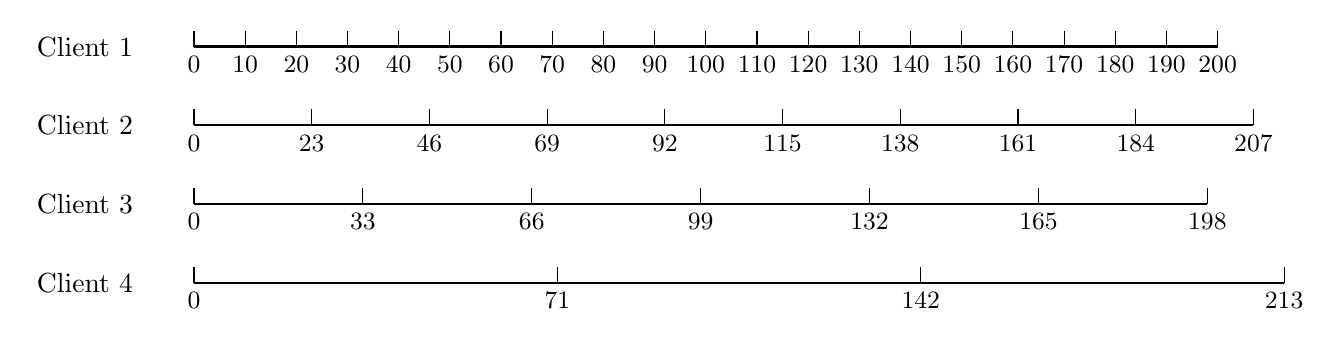
\begin{tikzpicture}[xscale=0.065]
        % Client 1
        \draw[thick] (0,4) -- (200,4);
        \foreach \x in {0,10,...,200} {
            \draw (\x,4) -- (\x,4.2);
            \node[below] at (\x,4) {\small \x};
        }
        \node[anchor=east] at (-10,4) {Client 1};
    
        % Client 2
        \draw[thick] (0,3) -- (207,3);
        \foreach \x in {0,23,...,207} {
            \draw (\x,3) -- (\x,3.2);
            \node[below] at (\x,3) {\small \x};
        }
        \node[anchor=east] at (-10,3) {Client 2};
    
        % Client 3
        \draw[thick] (0,2) -- (198,2);
        \foreach \x in {0,33,...,198} {
            \draw (\x,2) -- (\x,2.2);
            \node[below] at (\x,2) {\small \x};
        }
        \node[anchor=east] at (-10,2) {Client 3};
    
        % Client 4
        \draw[thick] (0,1) -- (213,1);
        \foreach \x in {0,71,...,213} {
            \draw (\x,1) -- (\x,1.2);
            \node[below] at (\x,1) {\small \x};
        }
        \node[anchor=east] at (-10,1) {Client 4};
    \end{tikzpicture}
    


    \end{document}
